\section{RICH-детектор эксперимента CBM}

%\todo \textbf{Может как-то сделать так, чтобы это описание CBM рича было после описания других ричей --- COMPASS, LHCb, HERA-b? Или как раз наоборот, лучше сразу после этой секции?}

%\todo \textbf{Перенести какую-то часть из секции RICHgeom}

По той причине, что в столкновении тяжёлых ионов рождается огромное количество заряженных $\pi$-мезонов, возникает необходимость идентифицировать электроны и позитроны.

Детектор черенковских колец (Ring Imaging CHerenkov detector, RICH) решает задачу идентификации частиц в диапазоне импульсов от до 8~\GeVoverC{}.
В паре с детектором переходного излучения TRD, покрывающем более высокие импульсы, RICH позволяет идентифицировать сигнальные электроны от лёгких векторных мезонов и $J/\psi$.

Фактор подавления пионов $\pi_{suppr}$ определяется как отношение количества восстановленных в STS треков, имеющих продолжение в геометрическом аксептансе детектора RICH, к количеству пионов, идентифицированных как электроны.

Для получения дилептонных спектров на SIS300 требуется $\pi_{suppr}$ порядка 10000, что осуществимо при совместном применении TRD и RICH, причём $\pi_{suppr}$ последнего должен составлять как минимум 100.

В случае SIS100 фон обусловлен такими источниками как $\gamma$-конверсия в мишени или распад $\pi^{0} \rightarrow \gamma + e^{+} + e^{-}$.



% Из диссера Копфера

%For SIS100 the background is already dominated by physical sources like $\gamma$-conversion in the target or $\pi^{0}$-Dalitz decays at a pion suppression factor of $10^3$ (see section 2.6). The electron identification covers the full angular acceptance of the CBM detector, i.e. from \SI{2.5}{\degree} to \SI{25}{\degree} in polar angle and full azimuthal coverage. In order to accommodate the bending of tracks in the dipole magnet, all detectors behind the magnetic field will be wider by a factor 1.5 compared to the height.


CBM RICH имеет $CO_{2}$ радиатор, который характеризуется коэффициентом преломления $n=1.00045$ при $T=0$ и $p=1$ атм.



%\todo остаётся?
%Порог черенковского свечения для пионов составляет $p=4.65$~\GeVoverC.

CBM RICH предсталяет собой классический RICH-детектор с газовым радиатором, с одним сферическим зеркалом и МА~ФЭУ в качестве фотодетекторов.


Аксептанс детектора, с учётом расширения по горизонтали из-за наличия магнитного поля, разводящего частицы, представляет собой конус \SI{0}{\degree}--\SI{25}{\degree} с вершиной в точке первичного взаимодействия, растянутый по горизонтали в 1.5 раза. Таким образом в плоскости XY угол составляет \SI{0}{\degree}--\SI{37.5}{\degree}.
% Перенесено из RICHgeom
Аксептанс детектора составляет $\SI{25}{\degree}$ по вертикали и $\SI{37.5}{\degree}$ по горизонтали. Длина отведённого под детектор пространства вдоль оси пучка составляет 1900~мм, при этом передняя плоскость находится на расстоянии 1800~мм от точки взаимодействия, а задняя, соответственно, на расстоянии 3700~мм. Ещё 100~мм перед RICH отводится под пространство для стыковки магнита, STS, RICH и пучковой трубы. Исходя из того факта, что зеркала должны полностью покрывать геометрический аксептанс, ширина детектора выбрана 5268~мм, а высота 4420~мм.

% Перенесено из RICHgeom
\begin{figure}[H]
\centering
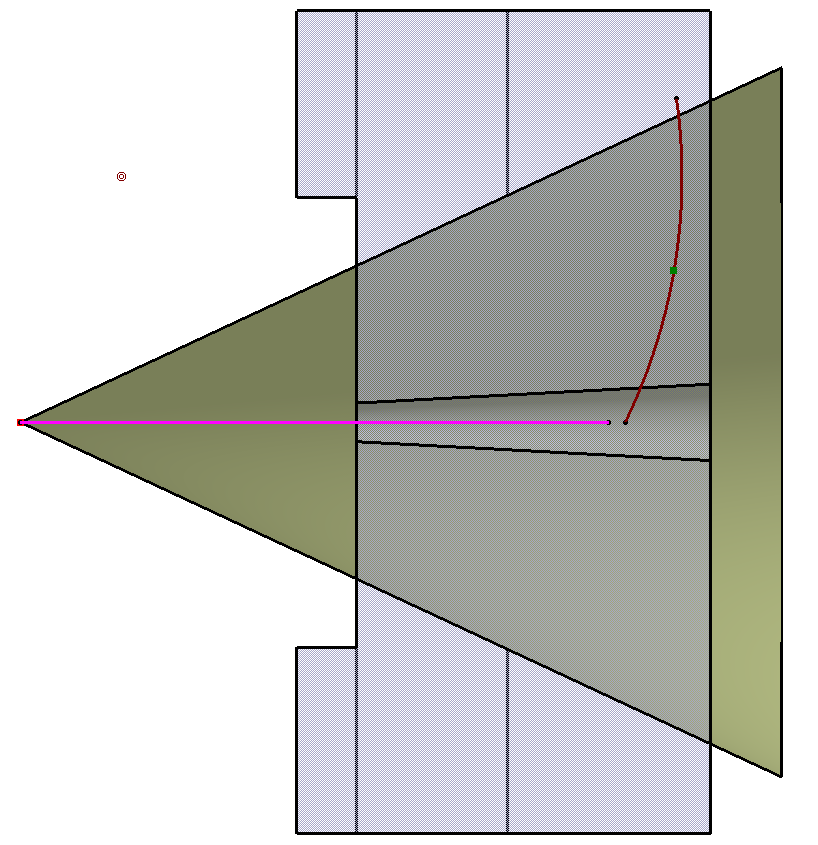
\includegraphics[width=0.7\textwidth]{pictures/RICH_construction.png}
\caption{Схема детектора CBM RICH, сид сбоку. Жёлтый конус -- геометрический аксептанс.}
\label{fig:RICHconstruction}
\end{figure}

% Перенесено из RICHgeom
На раннем этапе проектирования CBM RICH исходя из доступного пространства в общей экспериментальной установке было рассчитано, что фокусирующая система CBM RICH должна выполнять одно отражение с помощью двух сферических зеркал радиусом 3~метра, расположенных на расстоянии 3500~мм от точки взаимодействия. Рассматривался также вариант с двойным отражением, при этом вторая группа зеркал была плоская. Зеркала расположены симметрично относительно горизонтальной плоскости, проходящей через ось пучка, и полностью покрывают аксептанс детектора. Площадь каждого зеркала составляет приблизительно 7.5~м$^2$.

% Перенесено из RICHgeom
Для того чтобы выполнить требование к точности, зеркало такого радиуса технологически возможно изготовить только из сегментов. Рассматривались варианты изготовления различными компаниями, прототипы исследовались на \todo D0, Ronchi test, в итоге остановились на \todo.
Сегмент зеркала будет иметь размер около 40см$\times$40см. (точное значение указать невозможно, это ж не прямоугольник)

\subsection{Радиатор}

Разделение электронов и пионов в диапазоне импульсов до 10~\GeVoverC{} требует низкого коэффициента преломления радиатора, что определяет выбор углекислого газа в качестве радиатора. $CO_{2}$ имеет пороговый гамма-фактор $\gamma _{th} = 1 / \sqrt{1 - 1/n^{2}} = 33.3$, где $n = 1.00045$ --- коэффициент преломления при температуре $\SI{0}{\degreeCelsius}$, давлении 1000~мбар и длине волны 600~нм. Порог черенковского излучения для заряженных пионов составляет $p = 4.65$~\GeVoverC, а для электронов и позитронов --- $p = 0.03$~\GeVoverC. При этом порог для каонов $\approx 16$~\GeVoverC. \todo saturated черенковский угол для ультрарелятивистских частиц равен $\SI{1.72}{\degree}$. Полагая, что пионы и электроны могут быть разделены с эффективностью до 90\% \todo при максимальном черенковском угле $\theta = arccos(1/n)$, верхняя граница по импульсу при радиаторе из $CO_{2}$ получается $\approx$ 10~\GeVoverC.

% The separation of electrons and pions at momenta below 10~\GeVoverC requires a low refractive index of the radiator and therefore determines the radiator to be a gas. A $CO_{2}$ radiator is foreseen which has a threshold Lorentz factor of $\gamma _{th} = 1 / \sqrt{1 - 1/n^{2}} = 33.3$, given a refractive index of $n = 1.00045$ at a temperature of \SI{0}{\degreeCelsius}, a pressure of 1000~mbar, and a wavelength of 600~nm. The Cherenkov threshold is $p = 4.65$~\GeVoverC for charged pions and $p = 0.03$~\GeVoverC for electrons and positrons. The threshold for kaons is $\approx 16$~\GeVoverC. The saturated Cherenkov angle for ultrarelativistic particles is $\SI{1.72}{\degree}$. Assuming that pions can be separated from electrons up to 90\% of the maximum Cherenkov opening angle $\theta = arccos(1/n)$, electrons and pions can be separated up to $\approx$ 10~\GeVoverC with $CO_{2}$ as radiator gas.

Размер RICH-детектора определяется доступным пространством между кремниевой трековой станцией STS, расположенной внутри магнита, и детектором переходного излучения TRD. С одной стороны, высокая длина радиатора предпочтителька, т.к. она определяет высокий выход черенковских фотонов. С другой стороны чем меньше расстояние между последней станцией STS и первой станцией TRD, тем выше эффективность трекинга. Из этих соображений для RICH отведено пространство от 1800~мм до 3700~мм по оси пучка, не ограниченное по другим осям ничем, кроме пола. Перед RICH и за ним отведено ещё по 100~мм общего пространства для стыковки с STS и TRD. Зеркало расположено на расстоянии 3500~мм от точки взаимодействия, таким образом, рабочая длина радиатора составляет 1700~мм.

% The radiator length is 1.7~m and the volume $\approx 35 m^{3}$. Since the RICH detector will be placed between the STS in the dipole magnet and the TRD detector, its overall length is constrained by the distance between the magnet and its shielding yokes at about 1.6~m from target and the first TRD station. On the one hand, a long radiator is favourable due to the proportionality between photon yield and radiator length according to equation (2.8). On the other hand, a short gap between the tracking detectors STS and TRD is advantageous for tracking which requires a short RICH detector in between. In consequence, the overall length of the RICH detector including radiator, mirror, and support structure is foreseen to be $\approx 2$~m.

Нижняя граница длин волн при выборе радиатора определяется нижней границей длин волн чувствительности фотодетекторов

When designing a RICH detector ``one has to be extremely careful in matching the choice of (gas-)radiator with the sensitive wavelength range of the photon detection system'' [66]. In the case of the CBM-RICH, the low wavelength limit of the photomultiplier sensitivity (see section 3.4) coincides well with the absorption edge of $CO_{2}$ at $\approx 185$ nm (see section 6.2.1).

Явление chromatic absorption в $CO_{2}$ становится заметным только в области длин волн менее 200~нм и, следовательно, не ухудшает разрешения черенковского кольца.

%For $CO_{2}$, chromatic absorption becomes sizeable only in the region below 200 nm (see section 6.2.1) and does not deteriorate the Cherenkov ring resolution significantly as shown below.

Т.к. $CO_{2}$ не показывает высокого уровня сцинтилляции его часто добавляют в радиаторы, где другой газ является основным, в качестве гасящего газа. Ожидается около 5~фотонов/МэВ, в основном в синей области спектра. Энерговыделение в радиаторе порядка 1~\GeV ожидается при центральном $Au+Au$ столкновении, где рождается $\approx 1000$ минимально ионизирующих частиц, приводящих к $\approx 5000$ сцинтилляционных фотонов, летящих изотропно вдоль трека частицы. Если консервативно предположить, что 20\% фотонов достигает плоскости фотодетекторов и 25\% из них регистрируется, то в результате данного эффекта регистрируется дополнительно около $250$ фотонов, распределённых равномерно. При общем числе каналов порядка 55~000, указанный шум от сцинтилляции добавляет до 0.45\% \todo по всем каналам. Данный показатель находится в допустимом пределе и CBM RICH не теряет в эффективности.

%Due to the fact that $CO_{2}$ does not exhibit a high level of scintillation, it is often added to other radiator gases as quenching gas. Approximately 5 photons/MeV, mostly in the blue wavelength range, are expected [69]. An energy deposit in the radiator of $\approx 1$ GeV is expected for a central Au+Au collision with $\approx 1000$ minimum ionizing particles [6] leading to 5000 scintillation photons emitted isotropically along the particle tracks. This leads to $\approx 250$ measured additional photons distributed homogeneously over the photon detector plane when conservatively assuming that 20\% of the photons reach the photon camera with 25\% of them being detected. Given the total of 55 000 channels, noise from scintillation will add up to 0.45\% of all channels. This is well within the noise level that the CBM-RICH detector can tolerate without performance loss [6].

\subsection{Система фокусировки}

%The mirror of the CBM-RICH detector is split into two parts above and below the beam pipe. Each mirror half is oriented towards a photon detection plane and part of a sphere with R = 3.00 m. The total area of the two mirror halves is $12.96 m^2$ . The mirror halves consist of 36 mirror tiles each arranged in four rows of nine tiles. The tiles themselves have a slightly trapezoidal shape in order to minimise gaps in between to 3~mm to~4 mm. Two different tile sizes are foreseen, 430/425.6 mm $\times$ 425~mm for the inner two rows and 425.5/412.5~mm $\times$ 425~mm for the outer rows.

%The mirror tiles are made of a 6~mm thick SIMAX glass substrate front-coated with $Al+MgF_{2}$. Aluminium provides a good reflectivity in both the visible and the UV wavelength region down to below 200~nm. The $MgF_{2}$ layer is used as protective layer in order to prevent the formation of UV absorbing aluminium oxide. Mirror tiles from JLO Olomuc were successfully tested in a prototype (see section 5.1), characterised in terms of homogeneity [70] and reflectivity [71], and chosen to be used for the CBM-RICH detector.

%A tripod concept is foreseen for mounting the mirror tiles on an aluminum frame. Each mirror tile is glued to three actuators allowing for the precise alignment of the tiles in a sphere.

%In order to reduce the production of secondary particles, the material budget of the RICH detector has to be kept low. The mirror support structure is therefore designed as a compromise between stability and light weight.

% Перенесено из RICHgeom
В CBM RICH каждый сегмент зеркал будет крепиться на раме с помощью трёх \todo моторизированных актуаторов с удалённым управлением. Это позволяет корректировать положение отдельных сегментов 



\subsection{Фотодетекторы}

Задача фоточувствительной камеры CBM RICH --- детектировать черенковские фотоны, рождённые заряженными частицами в радиаторе и отражённые от зеркала. Камера разрабатывается для регистрации одиночных фотонов с высокой эффективностью. Для эффективного выполнения реконструкции необходима точная регистрация координат и времени прилёта каждого фотона.

%Task of the CBM-RICH photon camera is the detection of Cherenkov photons produced by charged particles in the gas radiator and reflected by the focusing mirror. The camera is developed for the detection of single photons with high efficiency. A precise measurement of position and time of arrival of each photon is required as input for the ring reconstruction algorithm discussed in section 2.5.3.

Фоточувствительная камера CBM RICH состоит из двух половин, расположенных над и под пучком в фокальной плоскости сферических зеркал. Обе половины находятся рядом с дипольным магнитом

%The photon camera of the CBM-RICH detector consists of two parts, one above and one below the beam pipe in the focal plane of the spherical mirrors. The two photon detector planes are located in front of the CBM dipole magnet shielded by the magnet yokes. The Cherenkov rings from the upper mirror half will be projected onto the upper photon detector, rings from the lower mirror half onto the lower photon detector. Each of the two photon detector planes is divided into two parts in order to optimise the angle towards the mirror. Thus, the camera consists of four separated areas, so-called camera modules. Each module covers an area of 0.6~m $\times$ 1.0~m (height $\times$ width). The total active camera area is $2.4 m^{2}$ .

%The CBM-RICH design foresees the usage of commercially available multianode photomultiplier tubes (MAPMTs) as photon sensors. The use of Micro Channel Plate (MCP) sensors is considered as alternative [6]. Due to the good geometrical coverage of these sensor types, no focusing elements like lenses or Winston cones are envisaged.

\subsection{Магнитное поле в области фоточувствительной камеры}

Моделирование распределения магнитного поля, созданного дипольным магнитом, с помошью пакета TOSCA показало, что фоточувствительная камера расположена в области, где паразитное поле составляет 10--50~мТл. Измерения показали, что для планируемой модели МА~ФЭУ эффективность регистрации одиночных фотонов значительно падает, если поле превышает уровень 1--2~мТл. Таким образом, магнитное поле в области фотосенсоров должно быть опущено до допустимого уровня.

% According to TOSCA 3 calculations, the photon camera is exposed to significant magnetic stray fields in the order of 10~mT to 50~mT. Measurements show that the single photon detection efficiency of the foreseen MAPMTs drops significantly for values exceeding 1~mT to 2~mT especially in the edge and corner pixels [6]. Therefore, the magnetic field strength in the region of the photon sensors has to be kept below this value.

Есть два способа уменьшить поле в области камеры --- повернуть зеркало и, следовательно, отодвинуть камеру от магнита, и поставить магнитный экран вокруг камеры. В CBM RICH была проведена оптимизация угла наклона зеркала точки зрения эффективности реконструкции и было решено спроектировать магнитный экран вокруг камеры.
Есть также третий вариант, который заключается во введении дополнительного отражения на пути черенковских фотонов. Этот подход, однако, был исключён, т.к. дополнительное отражение приводит к увеличению необходимой светочувствительной плоскости, а это значительно увеличивает стоимость детектора.

%In order to cope with the magnetic stray field in the region of the photon camera, two design options are considered and currently studied. The first option is to rotate the two mirror planes and to move the camera modules further away from the beam axis where the magnetic stray field is lower. In addition, a shielding box enfolding the camera modules can reduce the magnetic field strength in the region of the photocathodes significantly. The second option is the use of a second mirror reflecting the Cherenkov photons to the camera positioned farther away from the magnet. This option, however, requires a larger camera surface due to an increased focal length. Details on all design options can be found in [6].


%Ссылка на прогресс репорт 2015 стр. 53.

% Перенесено из RICHgeom
Положение фоточувствительной камеры в пространстве определяется относительно зеркал исходя из соображений эффективности регистрации колец. В CBM детектор RICH расположен непосредственно за дипольным магнитом, причём отражённые от сферических зеркал черенковские фотоны летят в направлении противоположном пучку. Уменьшение угла наклона зеркал теоретически приводит к повышению эффективности детектора, но на практике невозможно из-за нехватки пространства для размещения камеры в небольшом зазоре между магнитом и конусом аксептанса RICH. Увеличение угла наклона зеркал позволило бы вывести фотодетектор далее вверх из области магнитного поля, но это приводит к нежелательным оптическим эффектам, отрицательно влияющим на эффективность. Следовательно, камера должна быть расположена очень близко к дипольному магниту. Отсюда возникает необходимость экранировать камеру от магнитного поля, составляющего 50-100~мТл в области МА~ФЭУ. Рассчитано, что данное семейство МА~ФЭУ может работать в магнитном поле до 1~мТл без снижения эффективности.

\subsection{Характеристики детектора}

Ниже представлены результаты моделирования в среде CbmRoot в связке с генератором UrQMD, выполненные (\todo не мной!) с применением актуальной геометрической модели CBM RICH, построенной с помощью ``CATIA-GDML geometry builder'' и описанной в секции~\ref{sec:chapRICHgeo}.
Результаты показывают прирост по всем показателям по сравнению с геометрией, в которой каждая фоточувствительная камера моделируется двумя плоскостями, что даёт основание полагать, что цилиндрическая форма камеры более эффективна.

В CBM RICH выработано два типовых анализа модели детектора с помощью МК моделирования. В первом анализе в геометрической установке присутствует только RICH и он обстреливается одиночными электронами из точки первичного взаимодействия с импульсом и направлением из заданного диапазона. Такой анализ позволяет оценить выход черенковских фотонов, количество регистрируемых фотонов (хитов) (см.~\figref{fig:RICHchar1}), геометрический аксептанс детектора, а также параметры восстановленных колец.

Реконструкция колец в RICH состоит из двух этапов --- поиск колец, т.е. группировка хитов, принадлежащих одному кольцу (ring finding), и фитирование, т.е. определение параметров кольца (ring fitting), причём фитирование выполняется и окружностями и эллипсами.
МК моделирование позволяет не выполнять первый этап так, как это делалось бы на реальных данных, а принять за хиты одного кольца список хитов от фотонов, рождённых от рассматриваемого электрона (\todo parentID).
При этом второй этап индифферентен к истории хитов.
На~\figref{fig:RICHchar2} представлены распределения радиуса $R$ подобранного кольца, полуосей $A$ и $B$ подобранного эллипса. На~\figref{fig:RICHchar3} показаны распределения разброса хитов от кольца $dR$ и эллиптичности $B/A$.
Следует отметить, что в алгоритме поиска колец значение 7 выбрано как минимально допустимое количество хитов в кольце.
В случае МК моделирования с одиночными электронами возможна ситуация, когда количество хитов в кольце меньше~7 (см.~\figref{fig:RICHchar1} (справа)). Это означает, что такое кольцо теоретически есть, но не будет восстановлено. \todo формулировка

\begin{figure}[H]
\begin{minipage}[t]{0.495\textwidth}
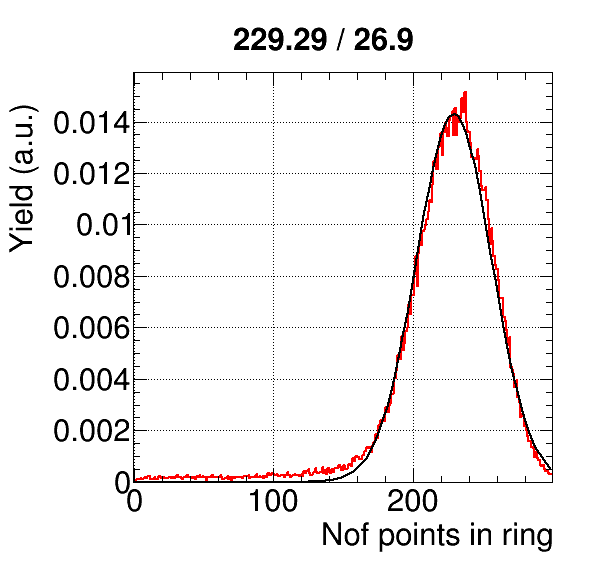
\includegraphics[width=0.9\textwidth]{pictures/RICH_nPoints_dist.png}
\end{minipage}
\begin{minipage}[t]{0.495\textwidth}
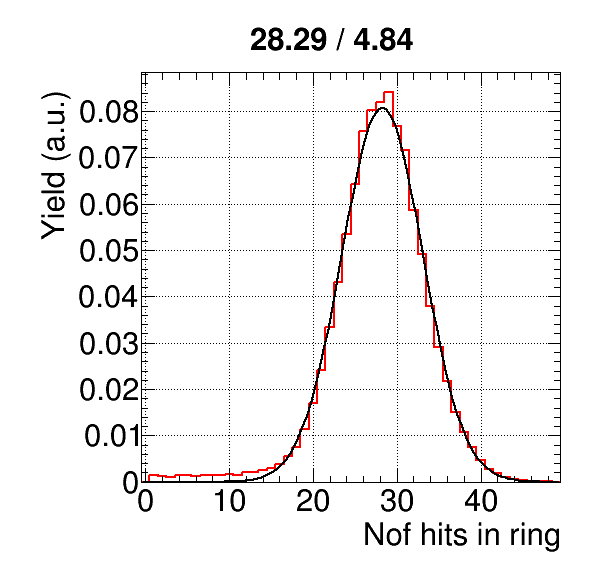
\includegraphics[width=0.9\textwidth]{pictures/RICH_nHits_dist.png}
\end{minipage}
\caption{}
\label{fig:RICHchar1}
\end{figure}

\begin{figure}[H]
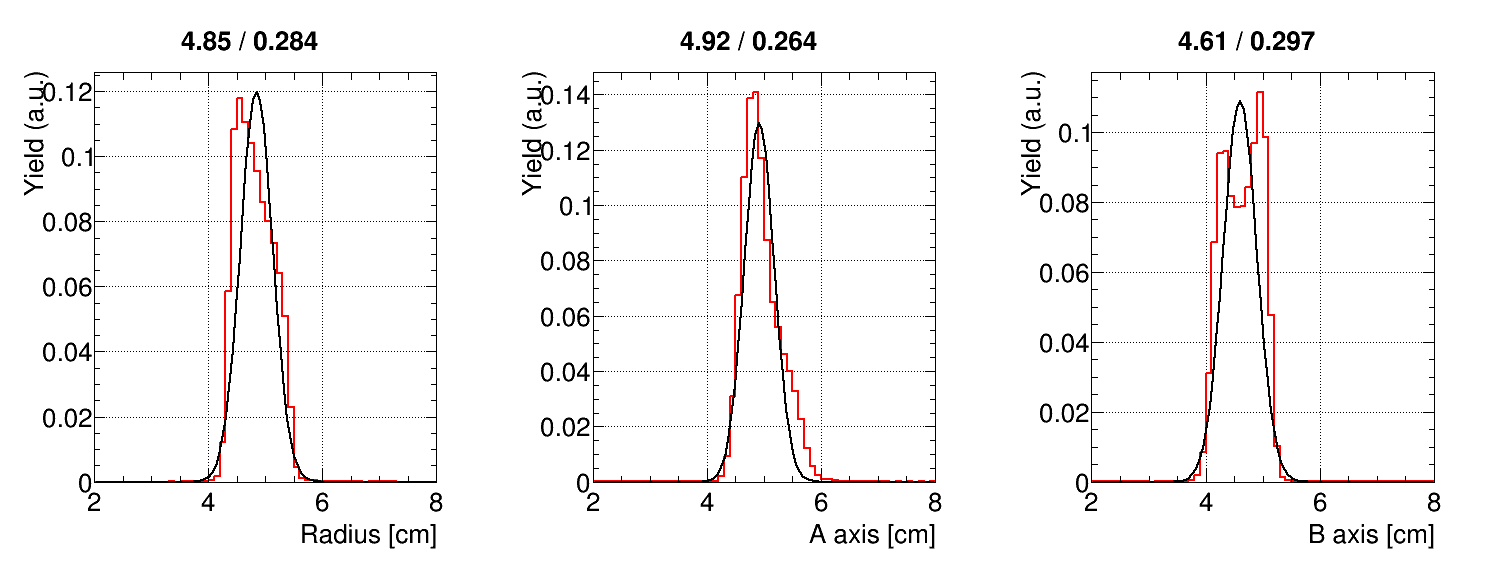
\includegraphics[width=0.95\textwidth]{pictures/RICH_R_A_B.png}
\caption{}
\label{fig:RICHchar2}
\end{figure}

\begin{figure}[H]
\begin{minipage}[t]{0.495\textwidth}
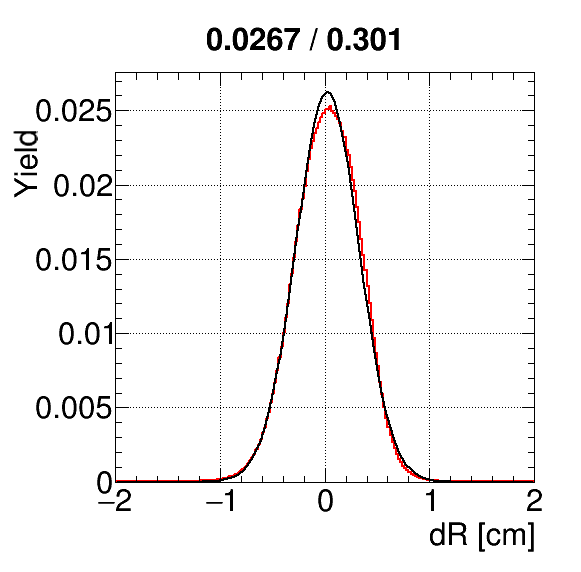
\includegraphics[width=0.9\textwidth]{pictures/RICH_dR.png}
\end{minipage}
\begin{minipage}[t]{0.495\textwidth}
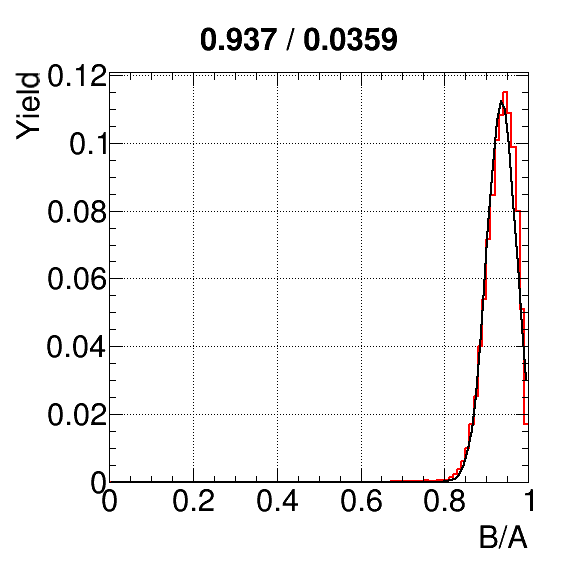
\includegraphics[width=0.9\textwidth]{pictures/RICH_BoverA.png}
\end{minipage}
\caption{}
\label{fig:RICHchar3}
\end{figure}

%Все значения - средние.
%Один электрон рождает 230 фотонов, из которых регистрируется 28 фотонов.
%Радиус кольца 4.85~см, отношение полуосей эллипсов $A/B=$0.937.


Второй анализ выполняется по результатам моделирования стандартного $Au+Au$ события CBM с помощью UrQMD. В этом случае есть две группы событий --- центральные столкновения при энергии 8~\GeVperNucl{}, характерные для SIS100, и 25~\GeVperNucl{}, характерные для SIS300.

Т.к. задача данного моделирования --- оценить функционирование детектора в реалистичной ситуации, в геометрической установке присутствуют STS и магнит. При этом присутствует магнитное поле и выполняется полная реконструкция треков в STS. На~\figref{fig:CbmRichOneEvent} представлено изображение на одной плоскости реконструкции от одного события $Au+Au$ 25~\GeVperNucl{}. Красные точки обозначают хиты, зелёные --- пересечение с плоскостью реконструкции RICH продолжений восстановленных треков STS, отражённых от зеркала.

\begin{figure}[H]
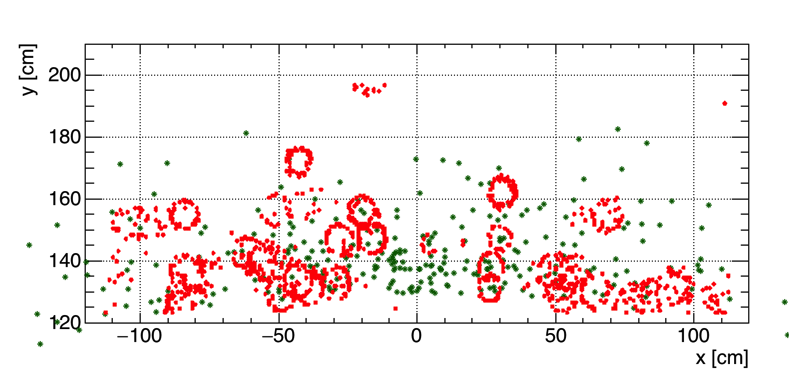
\includegraphics[width=0.9\textwidth]{pictures/CbmRichOneEvent.png}
\caption{Типовое событие (UrQMD, 25~\GeVperNucl{}) в одной фотодетектирующей плоскости RICH. Красные точки --- хиты RICH, зелёные --- продолжения треков STS.}
\label{fig:CbmRichOneEvent}
\end{figure}


\begin{table}[H]
\caption{}
\label{tabl:RICHAuAuChar}
\begin{tabular}{ | p{0.3\linewidth} | p{0.3\linewidth} | p{0.3\linewidth} | }
\hline
& 8~\GeVperNucl{} (SIS100) & 25~\GeVperNucl{} (SIS100) \\
\hline
$N_{hits}$ & 496 & 1431 \\
\hline
$N_{rings}$ ($\geq1$~хита) & 23.0 & 71.6 \\
\hline
$N_{rings}$ ($\geq7$~хитов) & 19.9 & 59.6 \\
\hline
\end{tabular}
\end{table}

\begin{figure}[H]
\begin{minipage}[t]{0.495\textwidth}
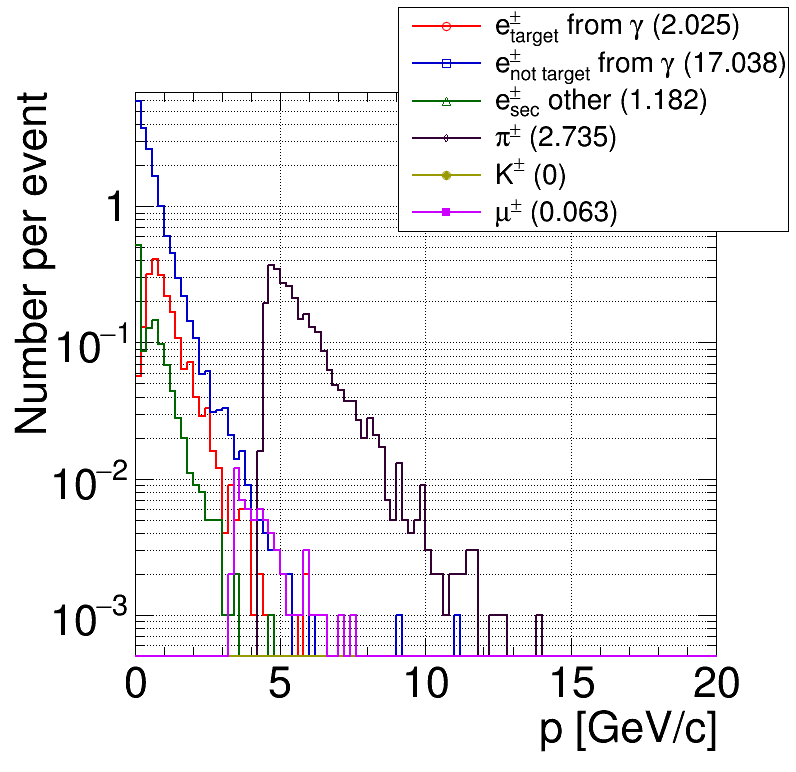
\includegraphics[width=0.9\textwidth]{pictures/RICH_8AGeV.png}
\end{minipage}
\begin{minipage}[t]{0.495\textwidth}
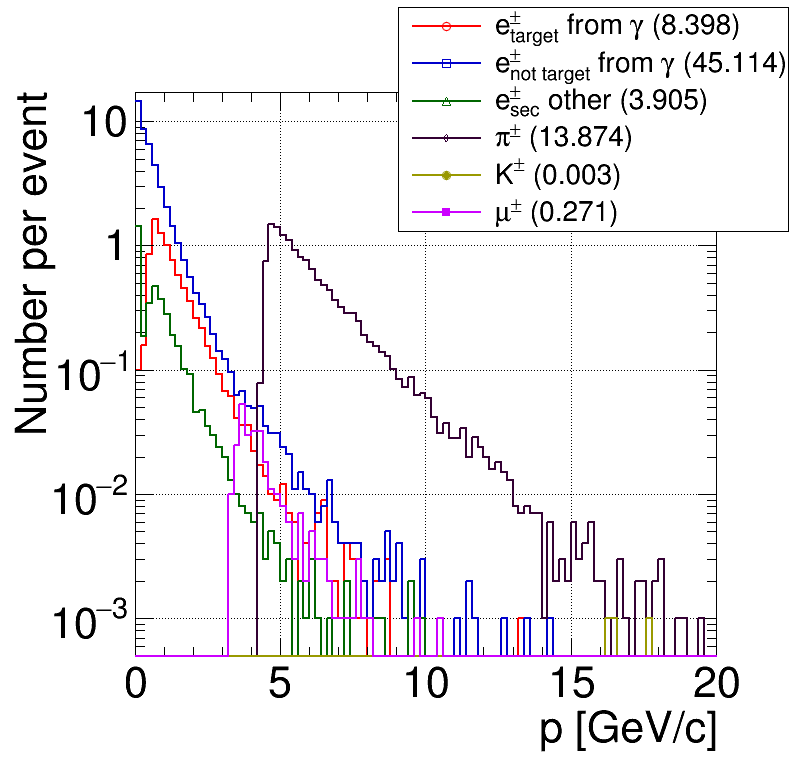
\includegraphics[width=0.9\textwidth]{pictures/RICH_25AGeV.png}
\end{minipage}
\caption{Основные типы частиц, регистрируемые в RICH при центральном $Au+Au$ столкновении при~8~\GeVperNucl{} (слева) и~25~\GeVperNucl{} (справа).}
\label{fig:RICH8and25AGeV}
\end{figure}

